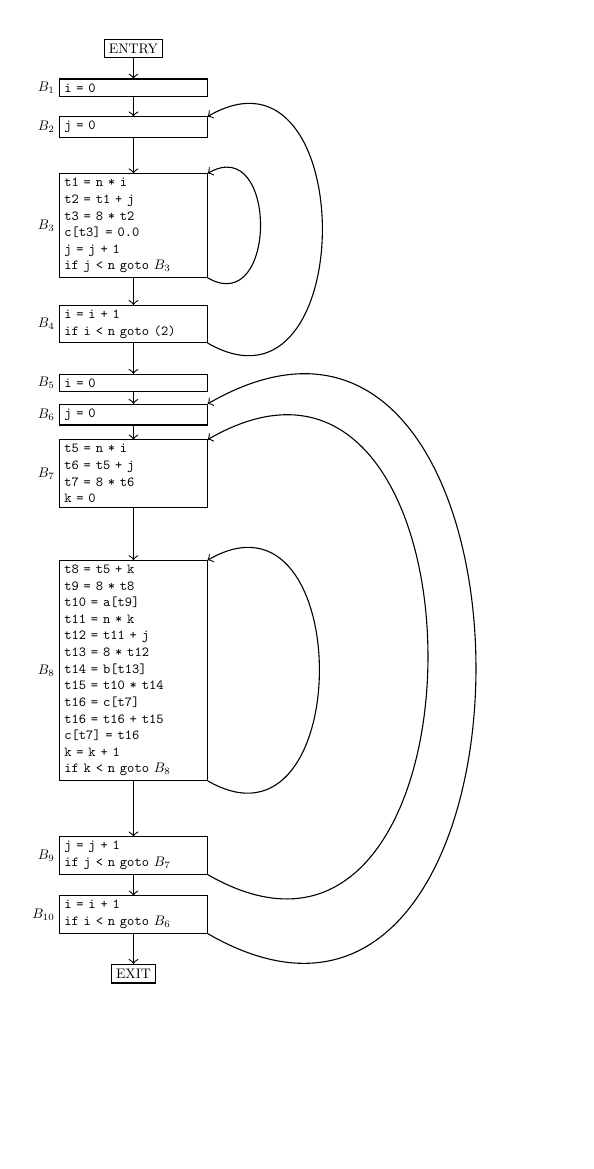
\begin{tikzpicture}[scale=0.5,every node/.style={scale=0.5}]
\tikzstyle{Block}=[draw, text width=10em, font=\ttfamily];
\tikzstyle{seq} = [->];
\tikzstyle{bender} = [bend right, out=-120, in=-60, looseness=2];
\node [Block,label=left:$B_1$] (v1) at (-0.5,2) {i = 0};
\node [Block,label=left:$B_2$] (v2) at (-0.5,1) {j = 0};
\draw [seq] (v1) edge (v2);
\node [Block,label=left:$B_3$] (v3) at (-0.5,-1.5) {\parbox{10em}{
t1 = n * i \\
t2 = t1 + j\\
t3 = 8 * t2\\
c[t3] = 0.0\\
j = j + 1\\
if j < n goto $B_3$}};
\draw [seq] (v2) edge (v3);
\node [Block,label=left:$B_4$] (v4) at (-0.5,-4) {\parbox{10em}{i = i + 1\\
if i < n goto (2)}};
\draw [seq] (v3) edge (v4);
\draw [bender] (v3.south east) edge[->] (v3.north east);
\draw [bender] (v4.south east) edge[->] (v2.north east);
\node [Block,label=left:$B_5$] (v5) at (-0.5,-5.5) {i = 0};
\draw [seq] (v4) edge (v5);
\node [Block,label=left:$B_6$] (v6) at (-0.5,-6.3) {j = 0};
\draw [seq] (v5) edge (v6);
\node [Block,label=left:$B_7$] (v7) at (-0.5,-7.8) {\parbox{10em}{t5 = n * i\\
t6 = t5 + j\\
t7 = 8 * t6\\
k = 0}};
\draw [seq] (v6) edge (v7);
\node [Block,label=left:$B_8$] (v8) at (-0.5,-12.8) {\parbox{10em}{t8 = t5 + k\\
t9 = 8 * t8\\
t10 = a[t9]\\
t11 = n * k\\
t12 = t11 + j\\
t13 = 8 * t12\\
t14 = b[t13]\\
t15 = t10 * t14\\
t16 = c[t7]\\
t16 = t16 + t15\\
c[t7] = t16\\
k = k + 1\\
if k < n goto $B_8$}};
\draw [seq] (v7) edge (v8);
\node [Block,label=left:$B_9$] (v9) at (-0.5,-17.5) {\parbox{10em}{j = j + 1\\
if j < n goto $B_7$}};
\node [Block,label=left:$B_{10}$] (v10) at (-0.5,-19) {\parbox{10em}{i = i + 1\\
if i < n goto $B_6$}};
\draw [seq] (v8) edge (v9);
\draw [seq] (v9) edge (v10);
\draw [bender] (v8.south east) edge[->] (v8.north east);
\draw [bender] (v9.south east) edge[->] (v7.north east);
\draw [bender] (v10.south east) edge[->] (v6.north east);
\node[draw] (v11) at (-0.5,3) {ENTRY};
\node[draw] (v12) at (-0.5,-20.5) {EXIT};
\draw [seq] (v11) edge (v1);
\draw [seq] (v10) edge (v12);
\end{tikzpicture}
